% TODO: Fix page numbering (placement and starting page).
\documentclass[
  12pt, 
  %draft
]{book}

\usepackage[
  linedheaders,
  parts,
  pdfspacing,
  eulermath,
  eulerchapternumbers,
  floatperchapter,
  listings,
  dottedtoc
]{classicthesis}
\usepackage[utf8]{inputenc}

\usepackage[
  inner=3cm,
  outer=2cm,
  top=2cm,
  bottom=2cm,
  includehead,
  includefoot
]{geometry}

\usepackage{graphicx}
\usepackage{xcolor}
\usepackage[numbers]{natbib}
\usepackage{setspace}
\usepackage{amsmath}
\usepackage{amsfonts}
\usepackage{algorithm}
\usepackage{algpseudocode}
\usepackage{mathtools}
\usepackage{lscape}
\usepackage[toc, page]{appendix}
\usepackage{bm}
\usepackage{afterpage}
%\usepackage{tabularx}
\usepackage{longtable}
\usepackage{quoting}

%Tikz packages.
\usepackage{tikz}
\usepackage{tikz-3dplot}
\usetikzlibrary{positioning}
\usetikzlibrary{bayesnet}

% For chapter abstracts.
\newenvironment{chapterabstract} {
  \begin{quoting}[font=itshape]
}{
  \hfill
  \end{quoting}
}

%Set double spacing.
\doublespacing

% Declare some math operators.
\DeclareMathOperator*{\argmin}{arg\,min}
\newcommand{\norm}[1]{\left\lVert#1\right\rVert_{2}}
\newcommand{\given}[1][]{\:#1\vert\:}
\newcommand{\std}[1]{{\footnotesize \( \pm \){#1}}}
\newcommand{\intd}[1]{{\mathrm d{#1}}}

\renewcommand{\bm}{\mathbold}

\setlength{\headheight}{23pt} 
\setlength{\footheight}{23pt} 

% Adjust align spacing.
\addtolength{\jot}{1.25em}

\pagenumbering{roman}

\title{
    {Dynamic SLAM, Object Reconstruction, Shape and Pose Prediction for 3D Scene Understanding}\\
    \vspace{15 mm}
    {\includegraphics[scale=1]{pre_chapters/figures/oxford_logo.png}\\
    {\large Department of Engineering Science\\ University of Oxford}\\}
}
\author{Jack Miles Hunt\\Kellogg College}

\date{Trinity Term 2018\\ This Thesis is submitted to the Department of Engineering Science, University of Oxford, for the 
degree of Doctor of Philosophy.
}

\bibliographystyle{ieeetr}

\begin{document}
\maketitle

\chapter*{Declaration}
I declare that the work contained in this Thesis is entirely my own, and except where otherwise indicated, 
describes my own research.

\chapter*{Acknowledgements}
I would first like to express my gratitude to the Engineering and Physical Sciences 
Research Council for their support of the Centre for Doctoral Training in Autonomous, 
Intelligent Machines and Systems, without which I could not have embarked on my DPhil 
journey. 

Additionally, I cannot understate my gratitude to the personnel of the AIMS 
CDT who from the very beginning have been supportive and encouraging. In particular, I 
would like to thank Wendy Adams for her personal support when I have faced difficulties 
and for introducing me to the Fish Finger Sandwich at the Royal Oak!

Of course, none of the work contained in this Thesis would have been possible without the 
support and guidance of my DPhil supervisors, Prof\@. Philip Torr and Prof\@. Victor Prisacariu. 
The work that they have overseen in their respective research groups has been a source of 
academic inspiration. Additionally, I would like to extend my thanks to Stuart Golodetz and 
Michael Sapienza, both of whom helped me immeasureably at the start.

Of course, my partner Zoe, my family and my friends must be noted here for their continued patience 
with me for the duration of my DPhil. I am sure that I have been difficult at times!

\chapter*{Abstract}
Advances in 3D computer vision have tremendously impacted the way that humans and computers interact,
ranging from immersive, Virtual Reality video games, to industrial robotics. Such applications of 3D 
vision are underpinned by a range of computer vision competencies, including pose estimation, mapping 
and semantic understanding. However, there remain many difficult, open research problems within the field, 
such as many common mapping approaches being restricted to static environments, the difficulty in obtaining 
high quality 3D models of objects, and scene understanding and modelling in large scale environments, such as 
towns or cities.

In this Thesis, there are three central subject matters that are approached. Firstly, an approach to the 
difficult task of dense mapping in dynamic environments is proposed. Central to the approach is a novel 
representation of the observed scene that allows for dynamic components, such as walking people to be 
separately handled from their static counterparts, such as furniture. It is demonstrated in this work that 
the proposed approach yields an improvement in pose estimation accuracy in dynamic scenes, versus it's 
common, static counterpart. Additionally, the proposed approach is capable of exceeding real-time performance, 
and may be leveraged for simple geometric feature extraction for semantics due to it's motion segmentation
capability.

The second central research topic of this Thesis is the high quality reconstruction of 3D objects. 
The approach to which comprises a novel representation and formulation of the problem, such that errors are 
corrected online. The proposed approach is evaluated against a state of the art method, over which an 
improvement in reconstruction is demonstrated. Additionally, the efficacy of the online correction procedure 
is demonstrated versus a vanilla approach. Finally, high levels of geometric accuracy are seen versus an appropriate 
benchmark.

%%% SPP
%%%%%% Preliminary results indicate ambitous task may be tractable
%%%%%% Promising avenue of research yada yada
The third major focus of this work is the simultaneous inference of object shape and pose in large scale, outdoor environments. 
An ambitous approach to regressing shape and pose in a weakly-supervised manner is presented, utilising a combination 
of Convolutional Neural Networks and Gaussian Processes. Early results indicate\dots

The work that is outlined in this Thesis is intended to provide a strong foundation for further research in the area of 
geometrically driven 3D scene understanding. However, immediate applications are evident. The motion segmentation and 
dense mapping approach for dynamic environments allows for larger scale dense mapping in previously prohibitive scenarios, 
and as such has applications in robotics. The object reconstruction work that constitutes the second major focus of the Thesis 
is applicable to the problem of collecting geometrically consistent 3D object data. Finally, the simultaneous inference of 
shape and pose is applicable to modelling scenarios of specific semantic interest, where an entire scene need not be reconstructed. 
The approach preliminarily demonstrates potential for large scale, semi-dense, geometric and semantic mapping.

\chapter*{Notation and Abbreviations Used}
\section*{Mathematical Notation}
This preliminary section introduces the mathematical notation used in this work. The following 
table outlines essential notational details, separated into sections on Sets, Fields and Groups, 
Linear Algebra, Sums and Products, Calculus and Probability Theory.
\begin{longtable}{p{.20\textwidth} | p{.8\textwidth}}
  \hline
  Symbolic Form & Meaning \\
  \hline
  \( \mathcal{A} \) & Calligraphic variables indicate mathematical sets (unless otherwise indicated).\\
  \( \{ a, b, c \} \) & A mathematical set consisting of the elements \( a \), \( b \) and \( c \).\\
  \( \{ a | \rho(a) \} \) & A mathematical set whose elements are defined by predicate \( \rho(a) \).\\
  \( a \in \mathcal{A} \) & The element \( a \), in the set \( \mathcal{A} \).\\
  \( f(a) \forall a \in \mathcal{A} \) & \( f(a) \) for all \( a \) in \( \mathcal{A} \).\\
  \( | \mathcal{S} | \) & Cardinality of \( \mathcal{S} \); the number of elements in \( \mathcal{S} \).\\
  \( \inf \mathcal{S} \) & Infimum of \( \mathcal{S} \).\\
  \( \sup \mathcal{S} \) & Supremum of \( \mathcal{S} \).\\
  \hline
  \( \mathbb{R}^{N} \) & The field of real numbers, of dimension \( N \).\\
  \( \mathbb{SE}(3) \) & The Special Eucledian Group of \( 4 \times 4 \) transform matrices.\\
  \( \mathbb{SO}(3) \) & The Special Orthogonal Group of \( 3 \times 3 \) rotation matrices.\\
  \hline
  \( \bm{A}\), \( \bm{\Theta} \) & Bold, uppercase symbols indicate matrix or tensor quantities.\\
  \( \bm{a}\), \( \bm{\theta} \) & Bold, lowercase symbols indicate vector quantities.\\
  \( \lVert \bm{a} \rVert_{n} \) & \( n \)-norm of a vector.\\
  \( \bm{a}^{T} \), \( \bm{A}^{T} \) & Transpose of a vector or matrix.\\
  \( \bm{A}^{-1} \) & The matrix inverse of \( \bm{A} \).\\
  \( \text{tr}(\bm{A}) \) & Trace of the matrix \( A \).\\
  \hline
  \(\sum_{a = 0}^{N} a\) & The sum from \( 0 \) to \( N \) of \( a \).\\
  \(\sum_{a \in \mathcal{A}}\) & The sum of the elements in \( \mathcal{A} \).\\
  \(\prod_{a = 0}^{N} a\) & The product from \( 0 \) to \( N \) of \( a \).\\
  \hline
  \( \frac{\partial f(\bm{a})}{\partial \bm{a}_{i}} \) & Partial derivative of \( f \) with respect to the \( i^{th} \) element of \( \bm{a} \).\\
  \( \nabla f(\bm{a}) \) & Gradient vector of \( f(\bm{a}) \). The vector of partial derivatives.\\
  \( \int f(a) \intd a \) & Infedinite integral over \( f(a) \) with respect to \( a \).\\
  \( \int_{m}^{n} f(a) \intd a \) & Definite integral over \( f(a) \) with respect to \( a \), between \( m \) and \( n \).\\
  \hline
  \( P(a, b, c) \) & Joint distribution over the random variables \( a \), \( b \) and \( c \).\\
  \( P(a \given b, c) \) & Distribution over the random variable \( a \), conditioned on \( b \) and \( c \).\\
  \( P(a) \) & Marginal distribution over the random variable \( a \).\\
  \( \mathcal{N}(a \given \mu, \sigma) \) & Gaussian distribution parameterised by mean \( \mu \) and standard deviation \( \sigma \).\\
  \( \mathcal{N}(\bm{a} \given \bm{\mu}, \bm{\Sigma}) \) & Multivariate Gaussian distribution parameterised by mean \( \bm{\mu} \) and covariance \( \bm{\sigma} \).\\
  \( \mathbb{E}(a) \) & Expectation over the random variable \( a \).\\
  \( b \sim P(a) \) & A sample \( b \), drawn from the distribution \( P(a) \).\\
  \( f(a) \sim \mathcal{GP}(a) \) & A function \( f(a) \), drawn from the Gaussian Process \( \mathcal{GP}(\bm{\mu}), \bm{\Sigma} \).\\
  \( \mathbb{KL}(P(a) \given P(b)) \) & KL Divergence from the distribution \( P(a) \) to the distribution \( P(b) \).\\
  \( \mathbb{JSD}(P(a) \given P(b)) \) & Jensen-Shannon Divergence between the distributions \( P(a) \) and \( P(b) \).
~\label{table:mathematical_notation}
\end{longtable}

\section*{Abbreviations}
In this preliminary section, a reference of abbreviations used in this work is given. The 
abbreviations and their associated meanings are given in the following table. Note that 
abbreviations that are used only in the literature review of Chapter~\ref{chap:lit_review} 
are excluded. Abbreviations are listed in order of first appearance in the text.
\begin{longtable}{p{.20\textwidth} | p{.8\textwidth}}
  \hline
  Abbreviation & Meaning \\
  \hline
  3D & Three Dimensional.\\
  VR & Virtual Reality.\\
  AR & Augmented Reality.\\
  RGB & Red-Green-Blue.\\
  RGBD & Red-Green-Blue-Depth.\\
  SLAM & Simultaneous Localisation and Mapping.\\
  AI & Artificial Intelligence.\\
  ML & Machine Learning.\\
  GPU & Graphical Processing Unit.\\
  SDF & Signed Distance Function.\\
  \hline
  TSDF & Truncated Signed Distance Function.\\
  ICP & Iterative Closest Points.\\
  ATE & Absolute Trajectory Error.\\
  RTE & Relative Trajectory Error.\\
  RMSE & Root Mean Squared Error.\\
  SVM & Suport Vector Machine.\\
  FPFH & Fast Point Feature Histogram.\\
  \hline
  CRF & Conditional Random Field.\\
  MLE & Maximum Likelihood Estimate.\\
  PDF & Probability Density Function.\\
  PMF & Probability Mass Function.\\
  CDF & Cumulative Density Function.\\
  PwP & Pixel-wise-Posteriors.\\
  PGM & Probabilistic Graphical Model.\\
  MAP & Maximum a Posteriori.\\
  CNN & Convolutional Neural Network.\\
  GP & Gaussian Process.\\
  GPLVM & Gaussian Process Latent Variable Model.\\
  DCT & Discrete Cosine Transform.\\
  IDCT & Inverse Discrete Cosine Transform.\\
  PCA & Principal Component Analysis.\\
  KL & Kullback-Leibler (Divergence).\\
  JSD & Jensen-Shannon Divergence.
~\label{table:abbreviations}
\end{longtable}

\tableofcontents
\listoffigures
\listoftables

\pagenumbering{arabic}

\chapter{Introduction}
~\label{chap:intro}
\begin{chapterabstract}
This introductory chapter outlines the motivation and background of this thesis, as well as it's objectives 
and structure.
\end{chapterabstract}

In recent years there has been much research activity in the field of 3D computer vision, a field concerned 
with the processing of 3D geometric data for machine vision. This work addresses a number of open technical 
challenges within the field of active, 3D vision. Specifically, the 3D reconstruction of dynamic environments, 
robust 3D reconstruction of arbitrary objects and the prediction of shape \& pose of objects. These areas of 
research are of interest to the computer vision community due to the broad application potential of such systems. 
Scene reconstruction for example, has applications ranging from mobile robotics to recreating the tangible world 
for Virtual Reality (VR) viewing. Object reconstruction has applications including the reproduction of tangible 
objects via 3D printing and building 3D object models for the training of machine learning systems. Finally, shape 
and pose prediction allows representations of a machine's environment to be inferred when traditional methods of 
reconstruction may not be feasible.

\section{3D Scene Reconstruction and Understanding}
~\label{sec:intro_scene_recon}
Driven by the availability of consumer grade depth sensing equipment such as the Microsoft Kinect RGBD sensor 
(introduced by Microsoft in 2009 for the XBox 360), there has been a renewed interest in dense scene reconstruction. 
Advances in recent years have allowed for the creation of digital reconstructions of the tangible world with 
consumer grade computer equipment~\cite{Newcombe2011,Kahler2016,Whelan2015}. Such systems iteratively integrate 
observed world points into a ``global'' model, such that over time, a smooth representation of the observed world 
surfaces is built. In addition to the integration of such information into a model, there is the task of inferring 
how the sensor has moved in world space, such that the observed points may be transformed and integrated into the 
appropriate model location. The amalgamation of these two tasks is known as SLAM (Simultaneous Localisation and Mapping). 
The basic SLAM pipeline is given in Figure~\ref{figure:basic_slam}. A typical reconstruction using such a system is given 
in Figure~\ref{figure:room_recon_example}.
\begin{figure}[!htbp]
  \centering
  \includegraphics[width=\linewidth]{figures/intro/basic_slam.pdf}
  \caption[Basic SLAM Pipeline]{A high level overview of the basic SLAM pipeline..}
~\label{figure:basic_slam}
\end{figure}

\begin{figure}[!htbp]
  \centering
  \includegraphics[width=.7\linewidth]{figures/intro/room_scene.png}
  \caption[Room Scale Dense Reconstruction]{An example of room-scale dense reconstruction.}
~\label{figure:room_recon_example}
\end{figure}

There has been much advancement in the 2D semantic scene understanding literature
~\cite{Girshick2014,Shelhamer2017,Civera2011}, which can be utilised within the context of 3D vision to introduce a 
semantic component to dense SLAM systems~\cite{Valentin2015,Golodetz2015,Cavallari2016}. Such a combination of techniques 
provides an adaptable component to AR and robotics applications. Early work on amalgamating the two areas of research have 
allowed one to view a reconstruction of their environment in VR and interactively label some of the objects within it, with 
the system inferring the remaining labelling's. An example of the output of such a system is given in Figure~\ref{figure:spaint_teaser}.
\afterpage{
  \begin{figure}[!htbp]
    \centering
    \includegraphics[width=.7\linewidth]{figures/intro/spaint-teaser.png}
    \caption[Room Scale Dense Reconstruction]{An example of semantic SLAM.\footnotemark}
~\label{figure:spaint_teaser}
  \end{figure}
~\footnotetext{Copyright \textit{Golodetz et al}, 2015.\\
\url{http://www.robots.ox.ac.uk/~tvg/projects/SemanticPaint/index.php}}
}

Though the results of the systems shown in Figures~\ref{figure:room_recon_example} and~\ref{figure:spaint_teaser} 
represent impressive advancements in computer vision, there are however open technical challenges. One such 
challenge is the successful modelling of real environments in which there are dynamic components (such as 
people walking in the camera's view). The traditional dense SLAM pipeline is unable to accurately build a 
globally consistent model in such environments. In addition, when using a combined reconstruction and 
semantics system such as that shown in Figure~\ref{figure:spaint_teaser}, many of the descriptive cues that 
enable the segmentation to be performed rely on features utilising 2D image information. As such, there is 
no ``true'' semantic 3D object learning and recognition.

As outlined, traditional dense SLAM systems have difficulty performing dense reconstruction in an 
environment where there is motion. The aforementioned sensor pose estimation phase in these systems
is prone to error or failure in such a scenario. The reason for this is due to the reliance on point based 
correspondences between frames. If a static environment is being modelled, then a high number of valid point 
correspondences will be found. However, when motion (independent of the sensors motion) is introduced into 
the scene, invalid correspondences may be found. For example, points that belong to a non moving object 
such as a chair may erroneously be matched to those on a moving scene component, such as a walking person.
Such erroneous correspondences can incur failure cases ranging from moderate model inconsistencies to total 
loss of sensor tracking\cite{Newcombe2015}.

Though there are many use cases for static scene reconstruction, the lack of robustness to dynamics is 
prohibitive in scenarios where a high level of machine perception is required. For example, if 
reconstructing a busy working environment in which there is a high level of dynamics (people walking, 
doors opening etc), an ideal reconstruction would not include artefacts of such motion. As such, the 
reconstruction system would be required to identify such components and account for them in the 
reconstruction process. Additionally, a system that is capable of detecting and segmenting such motion 
would be capable of extracting pertinent semantic information from such events.

\section{Object Reconstruction}
~\label{sec:intro_object_recon}
Modern machine learning provides much of the semantic and contextual information required to make meaningful 
inferences over the state of the world, as observed by a sensor (such as a camera). Much advancement 
has been made in recent years on the tasks of object detection and semantic segmentation, in standard 2D 
images~\cite{Girshick2014,Shelhamer2017,Civera2011}. However, there are many technical challenges that must be 
overcome before such efficacy on these tasks is reached for the 3D case. Many modern AI and machine learning algorithms 
require vast quantities of data to learn to perform a given task successfully. This is not prohibitive for systems that 
operate on standard 2D images, due to the abundance of available data. However, for the 3D case there is not a comparable 
volume of 3D data with real world geometric information from which a system can learn to perform complex tasks in the real 
world. One method of obtaining such geometric data is the reconstruction of objects, providing geometrically 
accurate models of real world objects.
% TODO: object reconstruction figure.

A related problem to that of sensor pose estimation as outlined in Section~\ref{sec:intro_scene_recon}, 
is pose estimation when performing reconstruction of individual objects. As with the larger scale case, point 
correspondences are problematic. One prominent reason is that for a smaller object versus a full scale scene 
(such as a room), there is less geometric data available in the former case than in the latter. As with the larger 
scale reconstruction, inconsistencies in the pose estimation phase can have varying effects on the resultant 
reconstruction. Such inconsistencies in the reconstruction can have a detrimental effect on learning based systems 
for 3D tasks if such inconsistent reconstructions are used to train such models. This is particularly troublesome as 
inconsistencies in object scale models in some cases have a more pronounced effect than in the case where 
an entire room is being reconstructed.

Though the model consistency problem for objects may be circumvented somewhat when using specialist equipment 
such as modelling turntables and laser range scanners, there are financial and practical issues that can be 
prohibitive. Thus, the ability to build high quality, consistent reconstructions of arbitrary objects with 
commodity depth sensing and computing hardware is desirable.

\section{Shape Prediction and Pose Prediction}
~\label{sec:intro_spp}
Though for many reconstruction scenarios the approaches outlined in Sections~\ref{sec:intro_scene_recon} 
and~\ref{subsec:intro_object_recon} are applicable, there are some situations in which the aforementioned 
approaches are not practical. For a complete, closed model, the reconstruction based approaches require that 
the object be fully observable, such that full coverage with the depth sensor is possible. As such, a clear 
failure point is the case in which the object is not fully observable, for example, when reconstructing a large 
object that is on a wall.

Additionally, the scene and object reconstruction approaches previously outlined depend on the iterative 
integration of observed range data. This approach may be troublesome in a scenario where an object may not 
be visible to the sensor for a sufficient period of time to build a smoothly reconstructed model. Circumventing 
this issue would require a very high framerate sensor. Additionally, the highly dynamic nature of such a scenario 
is likely to be problematic in a similar manner to outlined case of dynamic dense SLAM\@.

As such, a desirable approach to the 3D modelling of objects in problematic environments would not rely on 
direct reconstruction (in the sense of the integration of range data into a 3D model). Rather, an inference based 
approach is appropriate, due to the inherent stochasticity of building a full model of a partially observable 
object.

\section{Technical Aims and Thesis Structure}
~\label{sec:intro_aims_structure}
The aforementioned technical challenges pertain to the dense reconstruction of dynamic scenes, the 
reconstruction of objects and the reconstruction of objects for which no full view is available. As 
such, the following main research challenges are addressed in this work.
\begin{itemize}
  \item The dense reconstruction of dynamic environments.
  \begin{itemize}
    \item With real time performance.
    \item With comparable reconstruction quality to static counterpart.
    \item With an improvement in pose estimation over static counterpart.
  \end{itemize}
  \item Identifying the dynamic components of a scene.
  \begin{itemize}
    \item Utilising for semantics.
  \end{itemize}
  \item The reconstruction of arbitrary objects in a consistent manner.
  \begin{itemize}
    \item With comparable reconstruction quality to scene based alternative.
    \item With commodity hardware for wider applicability.
    \item Without known pose.
  \end{itemize}
  \item The inference of object centric scene properties where traditional reconstruction 
may not be possible.
  \begin{itemize}
    \item Inferring both shape and pose.
    \item Without requiring temporally consistent frames, averting tracking errors.
  \end{itemize}
\end{itemize}

With the central technical challenges of this work outlined, the remainder of this work is structured 
as follows. Firstly, Chapter~\ref{chap:lit_review} provides a comprehensive survey of the literature 
pertinent to this work. Initially, a survey of the dense SLAM (as introduced earlier in this chapter) 
literature is provided. The research outlined in this section is fundamental to much of the content of 
this work. Additionally, relevant works on semantics (such as semantic SLAM) are reviewed. 
Next is an assessment of relevant research on the topic of dynamics in 3D vision; topics include motion 
segmentation, optical and scene flow. Much of the material reviewed in this section is pertinent to the 
subject matter of Chapter~\ref{chap:moseg}. The next major area of research to be reviewed is on the topic 
of object reconstruction; relevant background to the topic of Chapter~\ref{chap:probobj}. Finally, 
Chapter~\ref{chap:lit_review} concludes with an assessment of the literature on the topics of pose prediction 
and shape prediction.

Chapter~\ref{chap:moseg} introduces the approach taken in this work to the problem of dense reconstruction 
in dynamic environments (environments with moving components). The chapter begins by outlining fundamental 
concepts in the static dense SLAM pipeline that shall be fundamental to much of the content in this work. 
Following this fundamental material, an approach to performing dense reconstruction and motion segmentation 
in dynamic scenes is presented. The method outlined in this chapter is evaluated against a state of the art 
dense SLAM system for static scenes, to which the presented approach demonstrates an overall improvement 
versus the static dense SLAM system. Additionally, the qualitative results of the presented approach 
demonstrate high quality resultant reconstructions on the test scenes. Furthermore, a demonstration of 
utilising motion segmentation to perform rudimentary object recognition using 3D geometric features is 
given.

Chapter~\ref{chap:probobj} introduces a novel approach to the segmentation and reconstruction of individual 
objects. The chapter outlines a novel Probabilistic approach to object reconstruction that reduces 
inconsistencies in pose estimation, which positively impacts the overall reconstruction quality. The 
approach presented in this chapter works with commodity computer and depth sensing equipment (though in 
principle it is trivially extendable, by design) and yields high quality reconstructions. Reconstruction 
quality is evaluated quantitatively and qualitatively against multiple alternative approaches. A 
quantitative evaluation of pose estimation quality is also provided, demonstrating an improvement over 
alternative approaches. The work in this chapter has been peer reviewed and published in the 
\textit{International Conference on 3D Vision (3DV)}. Additionally, the lead author \textit{Jack Hunt} 
presented a spotlight talk and poster at the event.

% -- "Stereo Shape and Pose Regression"
% ---- Outline approach; which questions addressed?
% ---- Outline experiments
% ---- Outline results
Chapter~\ref{chap:spp} approaches the problem of performing inference of shape and pose simultaneously. 
The work in this chapter is notably different in nature relative to the approaches taken in Chapters
~\ref{chap:moseg} and~\ref{chap:probobj}. The work in outlined in this chapter utilises a data driven, 
non-SLAM based approach to learn predictive models for shape and pose in a semi-supervised manner. A full 
view of the object of interest is not required, nor is temporal consistency between frames; ad-hoc prediction 
can be performed for arbitrarily sequenced frames.

\chapter{Literature Review}
%% Tracking and Mapping.
\section{Tracking and Mapping}
\label{sec:lit_review_tam}
Besl and McKay \cite{Besl1992}
\begin{itemize}
	\item 3D Shape Registration.
	\item Full 6DoF pose estimation.
	\item Requires shape complexity - geometrically distinctive.
	\item Compute closest point, compute \& apply registration, iterate until MSE low. 
	\item Convergence not guaranteed, determined empirically to be rapid over first few iterations.
\end{itemize}

Curless and Levoy \cite{Curless1996}
\begin{itemize}
	\item Early volumetric reconstruction work.
	\item Integrates aligned range images in to a volume.
	\item Volume introduced is SDF - cumulative and weighted.
	\item Isosurface extracted from SDF - Marching Cubes.
	\item Gaps filled by tesselation.
\end{itemize}

Zhou et.al. \cite{Zhou2008}
\begin{itemize}
	\item Alternative representation to Curless and Levoy.
	\item Massively parallel KD-Tree construction.
	\item Suitable for real-time use.
	\item Parallelism achieved by building tree with BFS.
	\item Example use given for Ray Tracing and Photon Mapping.
\end{itemize}

Censi \cite{Censi2008}
\begin{itemize}
	\item PL-ICP, ICP using point-to-line metric.
	\item Closed form solution in planar case.
	\item Quadratic convergence in finite amount of steps.
	\item New formulation weighted by normal and solved by reducing to quadratic form and introducing Lagrange Multipliers.
	\item Prior to optimisation, trimming procedure used to remove outliers.
\end{itemize}

Newcombe et.al. \cite{Newcombe2011}
\begin{itemize}
	\item Real time mapping of indoor scenes with Kinect sensor.
	\item Invariance to lighting.
	\item Observations fused in to SDF like volume of Curless et al - TSDF
	\item Multilevel ICP(coarse to fine) used to obtain pose.
	\item Measurement->integration->isosurface extraction->pose update.
	\item Limited to static scenes.
\end{itemize}

%TO-DO:fix name
Neissner et.al. \cite{NieBner2013}
\begin{itemize}
	\item Pipeline follows that of KinectFusion.
	\item Introduce a spatial Hashing data structure.
	\item TSDF split in to Voxel Blocks which are hashed.
	\item Low space and time complexity.
	\item Streaming system to reduce GPU memory usage.
\end{itemize}

Thomas et.al. \cite{Thomas2013}
\begin{itemize}
	\item Represent scene as a set of planes with attributes.
	\item Motivated by planar nature of objects such as tables and cabinets.
	\item Attributes are bump(normal) image for geometry encoding, mask image encoding confidence and RGB image.
	\item Rendering by quadrangulation. %Cite this
	\item Tracking as with KF - linearized GICP.
\end{itemize}

Salas-Moreno et.al. \cite{Salas-Moreno2013}
\begin{itemize}
	\item Introduce a new "Object Orientated" Dense SLAM paradigm.
	\item Incorporates prior knowledge that many scenes have repeated structure.
	\item Scene split in to graph of objects. Pose graph optimisation used.
	\item ICP run against object renderings, followed by detection and insertion of objects. Finally graph optimisation.
	\item Graph based re-localisation.
	\item Requires database of known objects.
\end{itemize}

%TO-DO:fix name
Stuckler et.al. \cite{Stuckler2014}
\begin{itemize}
	\item Uses multiple resolution, probabilistic surfel maps as representation. \cite{Pfister2000}
	\item Octree with spatial and appearance statistics at each level.
	\item Randomised loop closure - graph and key-view based.
	\item Pose estimation by maximising observation likelihood with uncertainty measure.
\end{itemize}

Salas-Moreno et.al. \cite{Salas-Moreno2014}
\begin{itemize}
	\item Exploits planar structure in the scene, like Thomas.
	\item Focus on detection and modelling of planes, refined over time.
	\item From generated Surfel maps, planes are segmented and holes filled over time. \cite{Pfister2000}
	\item Fern encoding used for relocalisation. %Reference Fern Encoding - Glocker et al
	\item ICP between measured vertex map and predicted vertex map.
\end{itemize}

Prisacariu et.al \cite{Prisacariu2014} Followed up by tech report \cite{Kahler2015}
\begin{itemize}
	\item Open source implementation of Voxel Hashing.
	\item A number of optimisations to the data structure(allocation \& integration) and raycaster.
	\item IMU data to supplement camera observations for tracking.
	\item 47Hz NVIDIA Shield tablet, 910Hz Titan X.
\end{itemize}

Whelan et.al \cite{Whelan2015}
\begin{itemize}
	\item Like KF but large scale(hundreds of meters), achieved using GPU cyclic buffers.
	\item Geometric and photometric camera pose constraints.
	\item Map updated by frame recognition, as-rigid-as-possible. %Reference as-rigid-as-possible
	\item Pose graph based loop closure.
\end{itemize}

Zhou et.al. \cite{Zhou2015}
\begin{itemize}
	\item Uses contour cues to improve camera tracking.
	\item Contour cues extracted from noisy and incomplete depth images.
	\item Correspondence constraints using scene geometry enforced on pose estimation.
	\item Based on KF pipeline.
	\item Depth image inpainting used before contour extraction.
\end{itemize}

%TO-DO: fix name.
Kahler et.al \cite{Kahler2016} 
\begin{itemize}
	\item Based on KF pipeline and InfiniTAM.
	\item Online submap alignment algorithm for drift correction.
	\item Inter-submap corrections based on graph optimisation.
	\item Loop closure detected using fern conservatories. %cite glocker
\end{itemize}

%% Semantic SLAM.
\section{Semantic SLAM}
\label{sec:lit_review_semantic}
Civera et.al. \cite{Civera2011}
\begin{itemize}
	\item Monocular EKF based SLAM.
	\item Semantics added to points via SURF correspondences with precomputed object descriptors.
	\item Geometric compatibility is then tested.
\end{itemize}

%TO-DO: fix name,
Stuckler et.al \cite{Stuckler2012} 
\begin{itemize}
	\item Uses RGB-D, not monocular.
	\item Fuses only detected objects.
	\item Object detection via random forests.
	\item Hand crafted features over object regions.
\end{itemize}

Valentin et.al. \cite{Valentin2015} Golodetz et.al. \cite{Golodetz2015}.
\begin{itemize}
	\item Online, real time semantic segmentation using user input.
	\item Dense reconstruction like KF.
	\item User physically interacts.
	\item Voxel Oriented Patch features using normals and appearance in CIELab.
	\item Streaming Random Forests\cite{Abdulsalam2007}  and Valentin version uses Mean Field \cite{Xing2002} optimised by \cite{Krahenbuhl2011}.
\end{itemize}

Bengio et.al. \cite{Bengio2013} - representation learning.
Girshick et.al \cite{Girshick2014} - feature hierarchies.
Handa et.al. \cite{Handa2015}
\begin{itemize}
	\item Real time reconstruction with semantic segmentation.
	\item Deep autoencoders stacked and trained on synthetic depth data.
	\item Uses depth only cues.
	\item KF style reconstruction.
\end{itemize}

Cavallari et.al. \cite{Cavallari2016}
\begin{itemize}
	\item Built on top of Voxel Hashing
	\item RGB frames passed to FCN\cite{Shelhamer2017}, PMF's out.
	\item Post rendering, colours determined by argmax over PMF bins.
	\item Texture(non label colours) trilinearly interpolated.
\end{itemize}

%% Dynamic SLAM.
\section{Dynamic SLAM, Motion Segmentation and Optical Flow}
\label{sec:lit_review_dynamic}
Tsap et.al. \cite{Tsap2000}
\begin{itemize}
	\item Algorithm for nonrigid motion tracking.
	\item Solve for dense motion vector fields between 3D objects via Finite Element Methods. %Cite FEM
	\item Iteratively analyses difference between actual and predicted behaviour.
	\item Iterative descent to find optimal parameters of nonlinear FEM.
	\item Tracking improved by using point correspondences.
	\item Not scene based.
\end{itemize}

Chen et.al \cite{Chen2011}
\begin{itemize}
	\item Nonrigid motion tracking applied to human body.
	\item Surface mesh extracted from multi view video and skinned.
	\item Hierarchical(w.r.t articulation) Weighted ICP is then applied.
	\item ICP points weighted by Approximate Nearest Neighbour %cite
	\item Prior human skeleton fitted.
	\item Not scene based.
\end{itemize}

Sun et.al. \cite{Sun2012}
\begin{itemize}
	\item Layered optical flow. Layered over detected moving objects.
	\item Depth ordered MRF's and Max Flow used for layering.%cite MF
	\item Number of layers automatically determined.
	\item Max Flow used to solve for discretised flow field cost function.
	\item Motion tracking only, no reconstruction.
\end{itemize}

Unger et.al. \cite{Unger2012}
\begin{itemize}
	\item Variational formulation for motion estimation and segmentation with occlusion handling.
	\item Parametric labelling of flow field for each object undergoing motion.
	\item Labels encoded with an MRF Potts model as with Sun. %cite potts model.
	\item Flow and labels solved for via Primal-Dual optimisation framework. %cite primal dual
	\item Again, motion only. No reconstruction.
\end{itemize}

Herbst et.al. \cite{Herbst2013}
\begin{itemize}
	\item Extension of Optical Flow to 3D scenes.
	\item Scene flow computed from RGB-D data, i.e. Kinect.
	\item Approach based on Brox et.al. \cite{Brox2004}
	\item Variational formulation and optimisation framework.
\end{itemize}

Stuckler et.al. \cite{Stueckler2013}
\begin{itemize}
	\item EM framework to segment rigid body motion from RGBD data.
	\item Robust to simultaneous fg and bg motion by treating both with parity.
	\item Sites of motion as well as motion params are posed as latent variables.
	\item No reconstruction, but feasibly could be extended.
\end{itemize}

Keller et.al. \cite{Keller2013}
\begin{itemize}
	\item Dense SLAM system capable of handling scene dynamics.
	\item Works with RGB-D data.
	\item Uses ICP outliers to determine dynamic scene components followed by flood fill.
	\item Surfel representation \cite{Pfister2000}
	\item Flat data structure. Does not have advantages of Voxel Hashing.
\end{itemize}

Perera et.al. \cite{Perera2015}
\begin{itemize}
	\item Motion segmentation in TSDF volumes,
	\item Based on MAP inference over a CRF on the TSDF.
	\item Can handle minor and major displacements.
	\item Motion labels and parameters found w.r.t. live frame and TSDF.
	\item $256^{3}$ voxel grid does not run real time. Scalability issues.
\end{itemize}

Newcombe et.al. \cite{Newcombe2015}
\begin{itemize}
	\item Handles non-rigidly deforming scenes.
	\item Built on KinectFusion pipeline.
	\item 6DoF motion field estimated that warps model to live frame.
	\item Warp field used to fuse new measurements in to canonical model.
	\item Warp field solved for by Dual Quaternion Blending. \cite{Kavan2006}
	\item Limitations, such as lack of robustness to open/closed topology changes(hands). Authors highlight scalability issues.
\end{itemize}

%% Object Reconstruction.
\section{Object Reconstruction}
\label{sec:lit_review_obj_recon}
Curless and Levoy \cite{Curless1996}
\begin{itemize}
	\item Object reconstruction from different viewpoints but statically.
	\item No pose tracking in the TAM sense.
\end{itemize}

Kolev et.al. \cite{Kolev2006}
\begin{itemize}
	\item Probabilistic 3D segmentation.
	\item Rather than direct reconstruction like Curless, the most probable image w.r.t. images is inferred.
	\item Level set representation used.
	\item Level set has analogous probability volume(pF,pB)
	\item Level set is evolved via a variational framework over probability volume.
	\item Only evaluated on synthetic data.
	\item Designed for objects with distinct appearance and homogeneous background, though some tolerance to noise is claimed.
\end{itemize}

Weise et.al. \cite{Weise2009}
\begin{itemize}
	\item 3D in hand scanning system.
	\item Point cloud representation, Surfel rendering. \cite{Pfister2000}
	\item Objects rotated in front of a sensor, suggests limited tracking ability.
	\item Drift offset in as-rigid-as-possible manner. %cite as-rigid-as-possible
	\item ICP registration. Topology graph used for deformation.
	\item Uses range scanner. No indication of RGBD capability. May need high quality equipment.
\end{itemize}

Ren et.al. \cite{Ren2013}
\begin{itemize}
	\item Probabilistic framework for tracking and reconstruction of objects.
	\item Initialised with a shape prior level set, which is then evolved as per observations.
	\item Works with RGBD data.
	\item Pixel-Wise-Posteriors used for segmentation. Prob volume like Kolev. \cite{Bibby2008}
	\item Experiments show limitations.
\end{itemize}

Dou et.al. \cite{Dou2015}
\begin{itemize}
	\item Reconstruction of deformable objects with a Kinect sensor.
	\item Loop closures automatically detected, distributing drift error over the loop.
	\item Latent shape and nonrigid deformation solved for with bundle adjustment.
	\item Surface represented as a triangular mesh.
	\item Experiments show high quality reconstructions, but with overnight run times.
\end{itemize}

Gupta et.al. \cite{Gupta2016}
\begin{itemize}
	\item 3D reconstruction and segmentation of objects with an RGBD sensor.
	\item Implicit representation, i.e. volumetric. Fusion with Softmax rather than weighted average like KF.
	\item Each voxel gets a label{obj, bg, empty}. Segmentation with graph cut and alpha expansion.
	\item Keyframe based loop closure.
	\item Pose estimation via photometric loss. Authors report drift to be a problem.
	\item Authors report difficulty in building a granular reconstruction.
\end{itemize}

%% Object Shape Prediction.
\section{Shape and Pose Prediction}
\label{sec:lit_review_prediction}

Prisacariu et.al. \cite{Prisacariu2011}
\begin{itemize}
	\item Shape prediction, segmentation(optimisation based) and pose optimisation.
	\item Hierarchical(early deep?) GPLVM's for Shape Latent Space Embedding. \cite{Lawrence2005}
	\item Unified energy function.
	\item Candidate shapes generated as one off regression in latent space.
\end{itemize}

Dame et.al. \cite{Dame2013}
\begin{itemize}
	\item Dense object reconstruction from monocular image source.
	\item Shape priors used to aid reconstruction and segmentation, GPLVM.
	\item Depth maps optimised for with Primal Dual with TV. Poses are known from PTAM.
\end{itemize}

Toshev et.al. \cite{Toshev2014}
\begin{itemize}
	\item Human pose estimation(articulated estimation) with Deep Neural Networks.
	\item Cascaded DNN regressors.
	\item No reconstruction, pose estimation only.
\end{itemize}

Wohlhart et.al. \cite{Wohlhart2015}
\begin{itemize}
	\item 3D object detection and pose recovery.
	\item CNN descriptors used with Nearest Neighbour Cost for detection and rough pose.
	\item Problem posed as KNN search in Descriptor Space.
	\item Object and Pose are coupled in training(i.e. two similar cars with different poses have distant descriptors)
\end{itemize}

Chang et.al. \cite{Chang2015}
\begin{itemize}
	\item Large scale dataset of 3D shapes.
	\item Synthetic data with no "source" sequence, i.e. no depth.
	\item Can be used to learn rich latent space embeddings.
\end{itemize}

Rock et.al. \cite{Rock2015}
\begin{itemize}
	\item Recovers a complete 3D model from a depth image of an object.
	\item Input depth image matched to database of objects via a Random Forest.
	\item Matched shape coarsely matched to depth map, then deformed at a higher granularity.
	\item Deformation manually optimised for.
\end{itemize}

Zhou et.al. \cite{Zhou2017_2}
\begin{itemize}
	\item Object detection from 3D Point Clouds.
	\item End-to-end trainable Convolutional, Region Proposal Network.
	\item Trained on KITTI LIDAR dataset. \cite{Geiger2013}
	\item Voxelisation of point cloud used for region detections.
\end{itemize}

Gwak et.al \cite{Gwak2017}
\begin{itemize}
	\item GAN like shape prediction with log-barrier ojective.
	\item Weakly supervised with sillhouettes and 3D shapes.
	\item May not work "in the wild"
\end{itemize}



\chapter{Real Time Motion Segmentation for Dense Volumetric Fusion}
%%% Local Variables: 
%%% mode: latex
%%% TeX-master: "../thesis"
%%% End: 

\section{Introduction}

\section{Related Work}

\section{Static Volumetric Fusion}

\section{Volumetric Fusion with Dynamic Scenes}

\section{Qualitative Results}

\section{Quantitative Results}

\section{Application to Semantic Scene Understanding}

\chapter{Probabilistic Object Reconstruction with Online Drift Correction}
%%% Local Variables: 
%%% mode: latex
%%% TeX-master: "../thesis"
%%% End: 

\section{Introduction}
Dense SLAM (Simultaneous Localisation and Mapping) has proven to be an effective
paradigm for the reconstruction of scenes of moderate size, with much research
on the topic driven by the availability of consumer grade depth sensing
equipment. However, there is a heavy reliance on descriptive geometry in the
scene when there is a lack of texture. Less descriptive geometry leads to an
increase in camera tracking error and causes model inconsistencies, especially
when a loop closure event occurs.

As object reconstruction can be seen as a smaller scale equivalent of the scene
based dense reconstruction problem, it too is prone to the tracking drift and
loop closure problem, sometimes to a prohibitive level. Often it may be
desirable to perform object reconstruction in an interactive way, for example,
as a component of a scene understanding system, or to procure training data for
the object in question.

With a high level of interaction comes an exacerbation of the aforementioned
shortcomings of dense SLAM, particularly due to the potential for frequent,
repetitive motion. This is the problem that is addressed in this chapter.

In this chapter, a probabilistic object reconstruction framework is presented
for the reconstruction of rigid objects based on object appearances.
The framework facilitates the correction of camera tracking drift by
representing the object to be reconstructed as a collection of overlapping
subsegments, such that deformations may be inferred to keep the subsegments
aligned, resulting in a consistent overall model. The system utilises a
volumetric representation for each of these object subsegments, as with many
larger scale reconstruction systems. Each voxel in the subsegments has
additional appearance posterior information pertaining to the voxels membership
of the object.

Over time, multiple volumes containing both surface and probabilistic appearance
information are maintained and manipulated to yield a robust and temporally
consistent model. Finally, the optimum object shape is optimised for within a
CRF (Conditional Random Field) framework.

The proposed system is inspired by\cite{Kolev2006} in that the representation
used for the shape of the object to be modelled is a volume of probabilities,
pertaining to posteriors over a voxels assignment to being either on the objects
surface or not. In the proposed system this volume of posterior probabilities is
``fused'' into with each frame, much like the fusion process in systems such as
KinectFusion\cite{Newcombe2011} and InfiniTAM\cite{Prisacariu2014}.

The probabilities that are ``fused'' into the volume are generated from an
appearance model, initialised prior to reconstruction by a Maximum Likelihood
procedure over the first frame of the RGB image. There are two appearance
models, one for the foreground object and one for the background, with the
foreground object indicated by a bounding box on the first RGB frame. A normal
distribution is fitted over the colour features of each class, foreground and
background. During the fusion process, the PDF's of these distributions are
evaluated on the latest colour observation for a voxel and posterior's are
computed and updated accordingly in the probability volume. Only those voxels
with a posterior higher for the foreground are rendered.

\section{Related Work}

\section{Algorithm Overview}
In the proposed system, the object model is divided into Subvolumes, each
consisting of a TSDF, colour volume and object Probability Volume. Additionally,
each has associated with it a Rigid Body Transform that specifies its pose
relative to the global coordinate frame.

At each time step, a segmentation model is applied to the RGB input image to
generate an object \textit{Probability Map} defining the segmented region to be
the object of interest and the remainder the background, to be discarded. Using
these generated Probability Maps, the system accumulates the probabilities into
the object \textit{Probability Volume} of the active Subvolume.

As with the Dense SLAM system outlined earlier in this work, the proposed system
also has \textit{Integration}, \textit{Tracking} and \textit{Rendering}
stages in it's pipeline(all of which are run at each time step). However, in
the proposed system, there are an additional two stages to the pipeline;
\textit{Online Model Correction} and \textit{CRF Based Segmentation}.

At the end of each frame, the online model correction algorithm is run, which
infers the relative poses between the subvolumes, mitigating tracking drift.
Once the reconstruction process is finished, we perform a CRF-based optimisation
to refine the resulting object segmentation over all Subvolumes.

The proposed approach is not tied to the use of any one probabilistic model,
though in the presented experiments PwP (Pixel Wise Posteriors) are used
\cite{Bibby2008}. An overview of the object reconstruction pipeline is shown in
Figure \ref{fig:probobj_pipeline_diagram}.

\begin{figure}[h]
  \label{fig:probobj_pipeline_diagram}
  \centering
  \includegraphics[width=\linewidth]{figures/object_recon/pipeline.pdf}
  \caption{The pipeline of the proposed Object Reconstruction approach.}
\end{figure}

\section{Probabilistic Formulation of Object Reconstruction}


\section{Online Model Correction}

\section{Volumetric Segmentation and Explicit Loop Closure Detection}

\section{Qualitative Results}

\section{Quantitative Results}

\chapter{Stereo Shape and Pose Regression}
\section{Introduction}
\label{sec:spp_introduction}
% Object reconstruction requires full view of object
% Relevant background - pose regression, shape regression
% In the wild, RGBD won't work, hence stereo.
% 

\section{Related Work}
\label{sec:spp_related}

\section{Algorithmic Overview}
\label{sec:spp_algorithm}
\subsection{Gaussian Process Marginal Likelihood}
\label{subsec:spp_gp_marginal_likelihood}
Given a Latent Variable Model of the following form
\begin{equation}
  \label{eqn:spp_gp_lvm}
  P(\bm{Y} \given \bm{X}, \bm{W}, \beta) = P(\bm{Y} \given \bm{WX}^{T}, \beta^{-1}\bm{I})
\end{equation}
Where in Equation \ref{eqn:spp_gp_lvm} the observed data $\bm{Y} \in \mathbb{R}^{N \times D}$ 
is mapped to a lower dimensionality manifold $\bm{X} \in \mathbb{R}^{N \times P}$, by parameters 
$\bm{W} \in \mathbb{R}^{P \times D}$ and variance $\beta$.

The marginal likelihood of $\bm{X}$ is of the form outlined in Equation \ref{eqn:spp_gp_marginal}.
\begin{equation}
  \label{eqn:spp_gp_marginal}
  P(\bm{Y} \given \bm{X}, \beta) = \int P(\bm{Y} \given \bm{X}, \bm{W}, \beta) P(\bm{W}) \intd{\bm{W}}
\end{equation}
Where in Equation \ref{eqn:spp_gp_marginal}, $P(\bm{W})$ is a Gaussian conjugate prior of the 
form $\mathcal{N}(\bm{W} \given \bm{0}, \bm{I})$.

To find the marginal distribution outlined in Equation \ref{eqn:spp_gp_marginal}, it's form may 
be simplified as follows in Equation \ref{}.
\begin{align}
  \label{eqn:spp_gp_marginal_simplify}
  % Line 1.
  P(\bm{Y} \given \bm{X}, \beta) &= \int \mathcal{N}(\bm{Y} \given \bm{WX}^{T}, \beta^{-1}\bm{I})
  \mathcal{N}(\bm{W} \given \bm{0}, \bm{I}) \intd{\bm{W}} \\
  % Line 2.
  &= \int \frac{1}{\sqrt{\left|2\pi\beta^{-1}\bm{I}\right|}} \exp{ 
  \Bigg[
    -\frac{\beta}{2} \big( \bm{Y} - \bm{WX} \big)^{T} \big( \bm{Y} - \bm{WX} \big) 
  \Bigg]}
  \frac{1}{\sqrt{\left|2\pi\bm{I}\right|}} \exp{ 
  \Bigg[
    -\frac{1}{2} \bm{W}^{T}\bm{W}
  \Bigg]} \intd{\bm{W}} \\
  % Line 3.
  &= \frac{1}{\sqrt{\left|2\pi\beta^{-1}\bm{I}\right|}} \frac{1}{\sqrt{\left|2\pi\bm{I}\right|}} 
  \int \exp{
  \Bigg[
    -\frac{\beta}{2} \big( \bm{Y} - \bm{WX} \big)^{T} \big( \bm{Y} - \bm{WX} \big) 
    -\frac{1}{2} \bm{W}^{T}\bm{W}
  \Bigg]} \intd{\bm{W}} \\
  % Line 4.
  &\propto \int \exp{
  \Bigg[
    -\frac{\beta}{2} \big( \bm{Y} - \bm{WX} \big)^{T} \big( \bm{Y} - \bm{WX} \big) 
    -\frac{1}{2} \bm{W}^{T}\bm{W}
  \Bigg]} \intd{\bm{W}} \\
  % Line 5.
  &\propto \int \exp{ 
  \Bigg[ -\frac{1}{2} \Big[
    \beta \big( \bm{Y} - \bm{X}^{T}\bm{W} \big)^{T} \big( \bm{Y} - \bm{X}^{T}\bm{W} \big) 
    + \bm{W}^{T}\bm{W}
  \Big] \Bigg]} \intd{\bm{W}} \\
  % Line 6.
  &\propto \exp{\Bigg[ -\frac{\beta}{2} \bm{Y}^{T}\bm{Y} \Bigg]} 
  \int \exp{
  \Bigg[ -\frac{1}{2} \Big[
    -\beta \big( \bm{Y}^{T}\bm{X}^{T}\bm{W} \big) 
    -\beta \big( \bm{W}^{T}\bm{XY} \big)^{T}
    +\beta \bm{W}^{T}\bm{XX}^{T}\bm{W}
    + \bm{W}^{T}\bm{W}
  \Big] \Bigg]} \intd{\bm{W}} \\
  % Line 7.
  &\propto \exp{\Bigg[ -\frac{\beta}{2} \bm{Y}^{T}\bm{Y} \Bigg]} 
  \int \exp{
  \Bigg[ -\frac{1}{2} \Big[
    -2\beta \bm{Y}^{T}\bm{X}^{T}\bm{W}
    +\beta \bm{W}^{T}\bm{XX}^{T}\bm{W}
    + \bm{W}^{T}\bm{W}
  \Big] \Bigg]} \intd{\bm{W}} \\
  % Line 7.
  &\propto \exp{\Bigg[ -\frac{\beta}{2} \bm{Y}^{T}\bm{Y} \Bigg]} 
  \int \exp{
  \Bigg[ -\frac{1}{2} \Big[
    \bm{W}^{T} \big( \beta \bm{XX}^{T} + \bm{I} \big) \bm{W}
    -2\beta \bm{Y}^{T}\bm{X}^{T}\bm{W}
  \Big] \Bigg]} \intd{\bm{W}}
\end{align}

\section{Qualitative Results}
\label{sec:spp_qualitative}

\section{Quantitative Results}
\label{sec:spp_quantitative}

\chapter{Discussion}
~\label{chap:discussion}
\begin{chapterabstract}
This chapter reviews the proposed algorithms in this work within the context 
of the initially outlined research objectives of this thesis.
\end{chapterabstract}

\section{Summary}
~\label{sec:discussion_summary}
This work has outlined novel approaches to various challenges in 3D computer vision, 
including handling dynamics in dense SLAM, reconstructing 3D objects and predicting both 
shape and pose. This chapter evaluates the methods, contributions and outcomes of these 
approaches, with the research objectives outlined in Section~\ref{sec:intro_aims_structure} 
as a point of reference.

This chapter proceeds as follows; first, Section~\ref{subsec:discussion_moseg} provides a 
summary of the dynamic SLAM and motion segmentation approach outlined in Chapter~\ref{chap:moseg}.
Following this, Section~\ref{subsec:discussion_probobj} provides a similar evaluation of the 
approach to object reconstruction outlined in Chapter~\ref{chap:probobj}. Section
~\ref{subsec:discussion_spp} evaluates the approach taken to shape and pose prediction in 
Chapter~\ref{chap:spp}.

Following the evaluations given in Sections~\ref{subsec:discussion_moseg},~\ref{subsec:discussion_probobj} 
and~\ref{chap:spp}, consideration is given to the limitations of the approaches of this work and potential 
future directions in Section~\ref{sec:discussion_limitations}. Finally, a high level conclusion and closing 
remarks are given in Section~\ref{sec:discussion_conclusions}.

\subsection{Real Time Motion Segmentation for Dense Volumetric Fusion}
~\label{subsec:discussion_moseg}
%-> Dense reconstruction with dynamics
%--> Aim to have KF like pipeline with dynamics
%---> Previously prohibitive due to...
%---> Results show...
%--> With RT performance
%--> TODO: measure this
%--> With comparable reconstruction quality
%--> With improved pose estimation
One of the central research objectives outlined in Section~\ref{sec:intro_aims_structure} 
is the development of an algorithm which facilitates the dense reconstruction of dynamic 
environments. As highlighted in Sections~\ref{sec:intro_scene_recon} and
~\ref{sec:lit_review_dynamic}, this has remained a challenging problem in 3D computer vision, 
due to the reliance on prominent pose estimation techniques on reliant point correspondences 
between frames. The novel approach taken in Chapter~\ref{chap:moseg} mitigates the restrictions 
incurred by this depencence by actively excluding dynamic scene components from the pose 
estimation phase of the pipeline, as shown in Figure~\ref{figure:moseg_pipeline}.

As demonstrated in Sections~\ref{sec:moseg_qualitative} and~\ref{sec:moseg_quantitative}, the 
approach taken demonstrates improvements in pose estimation quality over an open implementation
~\cite{Prisacariu2014} of the standard KinectFusion~\cite{Newcombe2011} pipeline when evaluated 
on the \textit{Dynamic Objects} subset of the TUM RGBD dataset~\cite{Sturm2012}. This improved 
performance is evident in Tables~\ref{table:moseg_ate} and~\ref{table:moseg_rte}, and 
Figures~\ref{figure:moseg_ate} and~\ref{figure:moseg_rte}. The improvement in the ability to 
accurately track sensor pose during reconstruction fulfils the research objective of designing 
an angorithm that provides an improvement in pose estimation versus static dense SLAM in dynamic 
scenes.

Additionally, it is evident from Section~\ref{sec:moseg_qualitative} that the proposed approach 
yields high quality reconstructions in dynamic environments that are comparable to their static 
counterparts when there is no motion in the scene. Again, this result is directly satisfying of 
the research objective to design a system that is capable of providing comparable quality 
reconstructions in previously troublesome environments.

%-> Identification/segmentation of moving objects
%--> Demonstrate potential for semantic use.

%-> Specific contributions.
%--> Novel expansion to classic KF pipeline
%--> Dual represenation, adaptive mu

%-> Impact of results
%--> Larger scale reconstructions with dynamics possible (vs dynamicfusion)
%---> Using volumetric representation and all it's advantages (versus non vol)
%---> Potential for application in larger, troublesome environments
%----> Industrial robotics

\subsection{Probabilistic Object Reconstruction with Online Drift Correction}
~\label{subsec:discussion_probobj}
%-> Dense reconstruction of objects
%--> Globally consistent
%---> As shown by results...
%---> Comparison to SoTA
%---> Previously problematic due to...
%----> As shown by results...
%--> Without known pose and with commodity hardware
%---> Initial aim of ease of use and applicability

%-> Impact of results.
%--> Globally consistent, dense reconstructions
%--> Runs without specialist hardware (unlike many current systems)
%--> Potential applications in data profcurement for deep learning etc

\subsection{Stereo Shape and Pose Regression}
~\label{subsec:discussion_spp}

\section{Future Work and Limitations}
~\label{sec:discussion_limitations}
%-> Though the contributions of this work..., future work...

%-> Moseg
%--> Limitations
%---> Currently maintains two full SDF's; this can be optimised
%---> Single "moving thing" class; can add more semantics
%--> Future work
%---> Optimise pipeline for better space complexity
%---> Introduce semantics throughout; multi moving things etc
%---> Expand to dynamic semantic slam system; a la spaint

%-> Object reconstruction.
%--> Limitations
%---> Purely observation driven; could better leverage stochastic framework
%---> Requires manual indication of object of interest
%--> Future work
%---> Expand probability framework to directly estimate missing geometry
%---> Exploit advances in saliency to remove manual indication requirement
%---> Multiple objects?

%-> General integration of moseg and object recon for super semantic slam

\section{Conclusions}
~\label{sec:discussion_conclusions}

\begin{appendices}
  \section{Mathematical Appendices}
~\label{appendix:mathematical}
%%% Local Variables: 
%%% mode: latex
%%% TeX-master: "../thesis"
%%% End: 
\label{appendix:mathematical}
\begin{landscape}
\subsection{Rodriguez Paramaterisation Partial Derivatives}
In this section the full Partial Derivatives of a Rotation Matrix $\mathbf{R}$
generated by the Formulation of Equation \ref{eqn:rodriguez_matrix_eq} in
Section \ref{subsec:moseg_static_camera_tracking} are given as follows.
\begin{equation}
  \label{eqn:rodrigues_full_alpha_deriv}
  \frac{\partial \mathbf{R}}{\partial \alpha} =
  % BEGIN SYMPY LATEX OUTPUT.
    \begin{bmatrix}
      - \frac{2 \alpha \left(\alpha^{2} - \beta^{2} - \gamma^{2} +
          1\right)}{\left(\alpha^{2} + \beta^{2} + \gamma^{2} + 1\right)^{2}} +
      \frac{2 \alpha}{\alpha^{2} + \beta^{2} + \gamma^{2} + 1} &
      - \frac{2 \alpha \left(2 \alpha \beta + \gamma\right)}{\left(\alpha^{2} +
          \beta^{2} + \gamma^{2} + 1\right)^{2}} + \frac{2 \beta}{\alpha^{2} +
        \beta^{2} + \gamma^{2} + 1} &
      - \frac{2 \alpha \left(2 \alpha \gamma - \beta\right)}{\left(\alpha^{2} +
          \beta^{2} + \gamma^{2} + 1\right)^{2}}
      + \frac{2 \gamma}{\alpha^{2} + \beta^{2} + \gamma^{2} + 1}\\
      -\frac{2 \alpha \left(2 \alpha \beta - \gamma\right)}{\left(\alpha^{2} +
          \beta^{2} + \gamma^{2} + 1\right)^{2}} + \frac{2 \beta}{\alpha^{2} +
        \beta^{2} + \gamma^{2} + 1} &
      \frac{2 \alpha \left(\alpha^{2} - \beta^{2} + \gamma^{2} - 1\right)}
      {\left(\alpha^{2} + \beta^{2} + \gamma^{2} + 1\right)^{2}} - \frac{2 \alpha}
      {\alpha^{2} + \beta^{2} + \gamma^{2} + 1} &
      - \frac{2 \alpha \left(\alpha + 2 \beta \gamma\right)}
      {\left(\alpha^{2} + \beta^{2} + \gamma^{2} + 1\right)^{2}} +
      \frac{1}{\alpha^{2} + \beta^{2} + \gamma^{2} + 1}\\
      - \frac{2 \alpha \left(2 \alpha \gamma + \beta\right)}{\left(\alpha^{2} +
          \beta^{2} + \gamma^{2} + 1\right)^{2}} + \frac{2 \gamma}{\alpha^{2} +
        \beta^{2} + \gamma^{2} + 1} &
      \frac{2 \alpha \left(\alpha - 2 \beta \gamma\right)}
      {\left(\alpha^{2} + \beta^{2} + \gamma^{2} + 1\right)^{2}} -
      \frac{1}{\alpha^{2} + \beta^{2} + \gamma^{2} + 1} &
      \frac{2 \alpha \left(\alpha^{2} + \beta^{2} - \gamma^{2} - 1\right)}
      {\left(\alpha^{2} + \beta^{2} + \gamma^{2} + 1\right)^{2}} - \frac{2 \alpha}
      {\alpha^{2} + \beta^{2} + \gamma^{2} + 1}
    \end{bmatrix}
    % END SYMPY LATEX OUTPUT.
\end{equation}

\begin{equation}
  \label{eqn:rodrigues_full_beta_deriv}
  \frac{\partial \mathbf{R}}{\partial \beta} =
  % BEGIN SYMPY LATEX OUTPUT.
  \begin{bmatrix}
    - \frac{2 \beta \left(\alpha^{2} - \beta^{2} - \gamma^{2} + 1\right)}
    {\left(\alpha^{2} + \beta^{2} + \gamma^{2} + 1\right)^{2}} - \frac{2 \beta}
    {\alpha^{2} + \beta^{2} + \gamma^{2} + 1} &
    \frac{2 \alpha}{\alpha^{2} + \beta^{2} + \gamma^{2} + 1} - \frac{2 \beta
      \left(2 \alpha \beta + \gamma\right)}{\left(\alpha^{2} + \beta^{2} +
        \gamma^{2} + 1\right)^{2}} &
    - \frac{2 \beta \left(2 \alpha \gamma - \beta\right)}{\left(\alpha^{2} +
        \beta^{2} + \gamma^{2} + 1\right)^{2}} - \frac{1}{\alpha^{2} + \beta^{2} +
      \gamma^{2} + 1}\\
    \frac{2 \alpha}{\alpha^{2} + \beta^{2} + \gamma^{2} + 1} - \frac{2 \beta
      \left(2 \alpha \beta - \gamma\right)}{\left(\alpha^{2} + \beta^{2} +
        \gamma^{2} + 1\right)^{2}} &
    \frac{2 \beta \left(\alpha^{2} - \beta^{2} + \gamma^{2} - 1\right)}
    {\left(\alpha^{2} + \beta^{2} + \gamma^{2} + 1\right)^{2}} + \frac{2 \beta}
    {\alpha^{2} + \beta^{2} + \gamma^{2} + 1} &
    - \frac{2 \beta \left(\alpha + 2 \beta \gamma\right)}{\left(\alpha^{2} +
        \beta^{2} + \gamma^{2} + 1\right)^{2}} + \frac{2 \gamma}{\alpha^{2} +
      \beta^{2} + \gamma^{2} + 1}\\
    - \frac{2 \beta \left(2 \alpha \gamma + \beta\right)}{\left(\alpha^{2} +
        \beta^{2} + \gamma^{2} + 1\right)^{2}} + \frac{1}{\alpha^{2} + \beta^{2} +
      \gamma^{2} + 1} &
    \frac{2 \beta \left(\alpha - 2 \beta \gamma\right)}{\left(\alpha^{2} +
        \beta^{2} + \gamma^{2} + 1\right)^{2}} + \frac{2 \gamma}{\alpha^{2} +
      \beta^{2} + \gamma^{2} + 1} &
    \frac{2 \beta \left(\alpha^{2} + \beta^{2} - \gamma^{2} - 1\right)}
    {\left(\alpha^{2} + \beta^{2} + \gamma^{2} + 1\right)^{2}} - \frac{2 \beta}
    {\alpha^{2} + \beta^{2} + \gamma^{2} + 1}
  \end{bmatrix}
  % END SYMPY LATEX OUTPUT.
\end{equation}

\begin{equation}
  \label{eqn:rodrigues_full_gamma_deriv}
  \frac{\partial \mathbf{R}}{\partial \gamma} =
  % BEGIN SYMPY LATEX OUTPUT.
  \begin{bmatrix}
    - \frac{2 \gamma \left(\alpha^{2} - \beta^{2} - \gamma^{2} + 1\right)}
    {\left(\alpha^{2} + \beta^{2} + \gamma^{2} + 1\right)^{2}} - \frac{2 \gamma}
    {\alpha^{2} + \beta^{2} + \gamma^{2} + 1} &
    - \frac{2 \gamma \left(2 \alpha \beta + \gamma\right)}{\left(\alpha^{2} +
        \beta^{2} + \gamma^{2} + 1\right)^{2}} + \frac{1}{\alpha^{2} + \beta^{2} +
      \gamma^{2} + 1} &
    \frac{2 \alpha}{\alpha^{2} + \beta^{2} + \gamma^{2} + 1} - \frac{2 \gamma
      \left(2 \alpha \gamma - \beta\right)}{\left(\alpha^{2} + \beta^{2} +
        \gamma^{2} + 1\right)^{2}}\\
    - \frac{2 \gamma \left(2 \alpha \beta - \gamma\right)}{\left(\alpha^{2} +
        \beta^{2} + \gamma^{2} + 1\right)^{2}} - \frac{1}{\alpha^{2} + \beta^{2} +
      \gamma^{2} + 1} &
    \frac{2 \gamma \left(\alpha^{2} - \beta^{2} + \gamma^{2} - 1\right)}
    {\left(\alpha^{2} + \beta^{2} + \gamma^{2} + 1\right)^{2}} - \frac{2 \gamma}
    {\alpha^{2} + \beta^{2} + \gamma^{2} + 1} &
    \frac{2 \beta}{\alpha^{2} + \beta^{2} + \gamma^{2} + 1} - \frac{2 \gamma
      \left(\alpha + 2 \beta \gamma\right)}{\left(\alpha^{2} + \beta^{2} +
        \gamma^{2} + 1\right)^{2}}\\
    \frac{2 \alpha}{\alpha^{2} + \beta^{2} + \gamma^{2} + 1} - \frac{2 \gamma
      \left(2 \alpha \gamma + \beta\right)}{\left(\alpha^{2} + \beta^{2} +
        \gamma^{2} + 1\right)^{2}} &
    \frac{2 \beta}{\alpha^{2} + \beta^{2} + \gamma^{2} + 1} + \frac{2 \gamma
      \left(\alpha - 2 \beta \gamma\right)}{\left(\alpha^{2} + \beta^{2} +
        \gamma^{2} + 1\right)^{2}} &
    \frac{2 \gamma \left(\alpha^{2} + \beta^{2} - \gamma^{2} - 1\right)}
    {\left(\alpha^{2} + \beta^{2} + \gamma^{2} + 1\right)^{2}} + \frac{2 \gamma}
    {\alpha^{2} + \beta^{2} + \gamma^{2} + 1}
  \end{bmatrix}
  % END SYMPY LATEX OUTPUT.
\end{equation}
\end{landscape}

  \section{Motion Segmentation Results Appendices}
~\label{appendix:moseg_additional_results}
  % TODO: Table numbering.
\subsection{Motion Segmentation figure: ATE results}
In this section, figure: results for the Motion Segmentation system
to complement those outlined in Section~\ref{sec:moseg_quantitative} are given.
The results in this section assess Absolute Trajectory Error on the TUM Dynamic
Objects \textit{Validation} set. Quantitative results are given in Table
~\ref{table:moseg_ate_validation} and visualised in Figure~\ref{figure:moseg_ate_validation}.

\begin{table}[!htbp]
\begin{center}
  \begin{tabular}{l c c}
    \emph{TUM Standard Sequence Name} & \emph{MoSeg} ATE (m) & \emph{Baseline} ATE (m) \\
    \midrule
    \textsf{fr3-sitting-static} & 0.044 & \textbf{0.030}\\
    \textsf{fr3-sitting-xyz} & \textbf{0.044} & 0.048 \\
    \textsf{fr3-sitting-halfsphere} & \textbf{0.026} & 0.028\\
    \textsf{fr3-sitting-rpy} & \textbf{0.043} & 0.044\\
    \textsf{fr3-walking-static} & \textbf{0.121} & 0.466\\
    \textsf{fr3-walking-xyz} & \textbf{0.082} & 0.633\\
    \textsf{fr3-walking-halfsphere} & \textbf{0.401} & 0.525\\
    \textsf{fr3-walking-rpy} & \textbf{0.073} & 0.561\\
  \end{tabular}
\end{center}
\caption[Motion Segmentation ATE Validation Set]
{The Absolute Trajectory Error (ATE) results (in metres, lower is better) 
achieved by the proposed approach in comparison to the baseline InfiniTAM
~\cite{Prisacariu2014} framework on a variety of the standard sequences from
  the TUM RGBD \textit{Validation} dataset~\cite{Sturm2012}. Results are in the
  format mean \( \pm \) standard deviation. The better result (by mean) on each
  sequence is highlighted in bold.}
~\label{table:moseg_ate_validation}
\end{table}

\begin{figure}[!htbp]
  \centering
  \includegraphics[width=0.95\linewidth]{figures/moseg/ate_validation.eps}
  \caption[Motion Segmentation ATE Validation Set]
  {Absolute Trajectory Error for the TUM Dynamic Scenes
    \textit{Validation} dataset.}
~\label{figure:moseg_ate_validation}
\end{figure}

\subsection{Motion Segmentation figure: RTE results}
In this section, figure: results for the Motion Segmentation system
to complement those outlined in Section~\ref{sec:moseg_quantitative} are given.
The results in this section assess Relative Trajectory Error on the TUM Dynamic
Objects \textit{Validation} set. Quantitative results are given in Table
~\ref{table:moseg_rte_validation} and visualised in Figure
~\ref{figure:moseg_rte_validation}.

\begin{table}[!htbp]
\begin{center}
  \begin{tabular}{l c c}
    \emph{TUM Standard Sequence Name} & \emph{MoSeg} RTE (m) & \emph{Baseline} RTE (m) \\
    \midrule
    \textsf{fr3-sitting-static} & \textbf{0.011} & \textbf{0.011}\\
    \textsf{fr3-sitting-xyz} & \textbf{0.031} & 0.034\\
    \textsf{fr3-sitting-halfsphere} & 0.024 & \textbf{0.022}\\
    \textsf{fr3-sitting-rpy} & 0.051 & \textbf{0.048}\\
    \textsf{fr3-walking-static} & \textbf{0.083} & 0.163\\
    \textsf{fr3-walking-xyz} & \textbf{0.067} & 0.285\\
    \textsf{fr3-walking-halfsphere} & \textbf{0.167} & 0.211\\
    \textsf{fr3-walking-rpy} & \textbf{0.121} & 0.194\\
  \end{tabular}
\end{center}
\caption[Motion Segmentation RTE Validation Set]
{The Relative Trajectory Error (RTE) results (in metres, lower is better) 
achieved by the proposed approach in comparison to the baseline InfiniTAM
~\cite{Prisacariu2014} framework on a variety of the standard sequences from
the TUM RGBD \textit{Validation} dataset~\cite{Sturm2012}. Results are in the
format mean \( \pm \) standard deviation. The better result (by mean) on each
sequence is highlighted in bold.}
~\label{table:moseg_rte_validation}
\end{table}

\begin{figure}[!htbp]
  \centering
  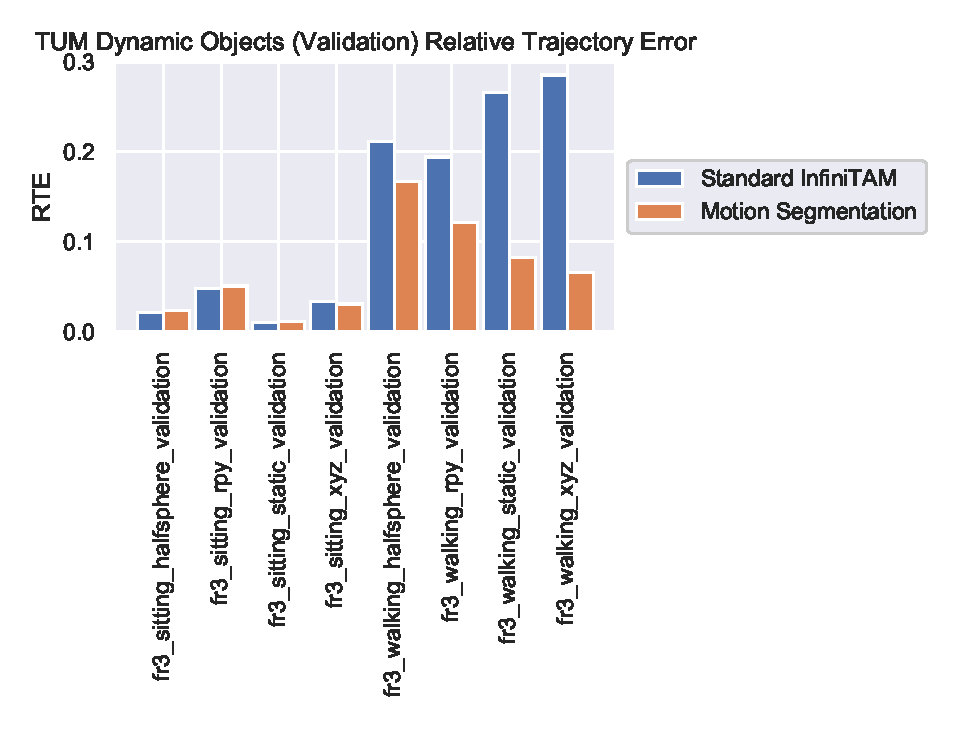
\includegraphics[width=0.95\linewidth]{figures/moseg/rte_validation.eps}
  \caption[Motion Segmentation RTE Validation Set]
  {Relative Trajectory Error for the TUM Dynamic Scenes
    \textit{Validation} dataset.}
~\label{figure:moseg_rte_validation}
\end{figure}
\end{appendices}

\bibliography{bib/definitions,bib/books,bib/slam_moseg,bib/segmentation,bib/objects,bib/ml}
\end{document}